\documentclass[12pt, a4paper]{report}
\usepackage[utf8]{inputenc}
\newcommand\preamble{
    \usepackage[italian]{babel}
    \usepackage{geometry}
    \usepackage{amsmath}
    \usepackage{amssymb}
    \usepackage{graphicx}
    \usepackage{ulem}
    \geometry{margin=2cm}
    \usepackage{listings}
    \usepackage{xcolor}
    \let\olditemize\itemize
    \renewcommand\itemize{\olditemize\setlength\itemsep{0em}}
}
% Definizione delle variabili
\newcommand{\imagePath}{Immagini/logoUni.png}

% Definizione del comando per la pagina di titolo con argomenti
\newcommand{\customTitlePage}[2]{
    \newcommand{\courseTitle}{#1}
    \newcommand{\academicYear}{#2}
    
    \begin{titlepage}
        \centering
        \includegraphics[width=0.5\textwidth]{\imagePath}\par\vspace{1cm}
        {\scshape\LARGE University of Studies of Genoa \par}
        \vspace{1.5cm}
        {\huge\bfseries \courseTitle \par}
        \vspace{2cm}
        {\Large\itshape Lorenzo Vaccarecci \par}
        \vfill
        \academicYear
    \end{titlepage}
}

\preamble

\begin{document}
\customTitlePage{Computer Security}{2024-2025}
\newpage
\tableofcontents
\chapter{Introduzione}
\section{Information Security}
\begin{itemize}
    \item La sicurezza concerne la protezione degli \textbf{asset} dalle \textbf{minacce (threats)}
    \item I proprietari (\textbf{owners}) valorizzano i loro asset e vogliono  proteggerli
    \item I proprietari analizzano le minacce e valutano i rischi. Questo aiuta la selezione di \textbf{contromisure} che riducono le \textbf{vulnerabilità}
\end{itemize}
\begin{equation*}
    Risk_{E} = P(E) \cdot I_{E}
\end{equation*}
Dove $E$ è l'evento che rappresenta la minaccia, $P(E)$ è la probabilità che l'evento si verifichi e $I_{E}$ è l'impatto che l'evento ha.
\begin{equation*}
    Risk_{Tot} = \sum_{e\in E} (P(e) \cdot I_{e})
\end{equation*}
$P(\cdot)$ può essere:
\begin{itemize}
    \item 0.7 - 1 : Alta
    \item 0.4 - 0.7 : Media
    \item $\leq 0.3$ : Bassa
\end{itemize}
\section{Security Properties}
\begin{itemize}
    \item Confidentiality: l'informazione non è conosciuta da non autorizzati, bisogna permettere solo a chi ne ha diritto attraverso \textbf{security policies}. Qualche volta si dice \textbf{privacy} per gli individui, \textbf{secrecy} per le organizzazioni, \textbf{anonymity} invece per nascondere l'identità.
    \item Integrity: l'informazione non deve essere modificata in modo malizioso.
    \item Authentication: i dati o i servizi devono essere accessibili solo da chi autorizzato. Solitamente il metodo di autenticazione è qualcosa che si ha, qualcosa che si conosce o qualcosa che sei (impronta digitale, firma, biometrica).
    \item Availability: i dati o i servizi devono esere accessibili e utilizzabili in qualsiasi momento. Questo significa che bisogna prevenire da attacchi DoS (\textbf{Denial of Service})
    \item Accountability: le azioni sono registrare e rintracciabili dalle parti responsabili.
\end{itemize}
\section{Protection Countermeasures}
\begin{itemize}
    \item Prevention: prevenire gli attacchi attraverso la progettazione di sistemi e impiegando tecnologie di sicurezza.
    \item Detection: i metodi principali sono il \textbf{logging} e il \textbf{MACs} (file hash per rilevare alterazioni).
    \item Response: varia dal ripristinare backup all'informare le autorità competenti o le parti coinvolte.
    \item Remediation
\end{itemize}
\section{Managing security: implementing a solution}
\begin{itemize}
    \item Security Analysis: analizza le minacce che potrebbero compromettere l'asset e propone delle politiche e soluzioni a costi appropriati.
    \item Threat Model: documenta le possibile minacce al sistema, immaginando tutte le possibili vulnerabilità che possono essere sfruttate.
    \item Risk Assessment: valutazione quantitativa dei rischi.
    \item Security Policy: per ogni rischio si descrivono le contromisure da adottare.
    \item Security Solution: progettazione e implementazione delle tecnologie appropriate a costi appropriati.
\end{itemize}
\chapter{Introduzione alla Crittografia}
\section{Concetti base}
CIA: Confidentiality, Integrity, Authentication
\begin{itemize}
    \item Confidentiality: l'informazioe rimane segreta
    \item Integrity: l'informazione non è alterata
    \item Authentication: i principali (Alice e Bob) sanno con chi stanno parlando  
\end{itemize}
\begin{itemize}
    \item Cryptology: lo studio di scritture segrete
    \item Steganography: la scienza di nascondere un messaggio in un altro messaggio
    \item Cryptography: la scienza di scrivere in modo segreto
\end{itemize}
\section{Schema generale della crittografia}
\begin{center}
    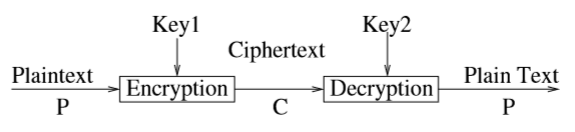
\includegraphics[width=0.5\textwidth]{Immagini/schemacrittografia.png}
\end{center}
Dove $E_{key_{1}}(P)= C$ e $D_{key_{2}}(C) = P$.
\begin{itemize}
    \item \textbf{\textcolor{red}{La sicurezza dipende dalla segretezza (secrecy) della chiave non dell'algoritmo}}
    \item Algoritmi Simmetrici: le due chiavi sono uguali oppure sono facilmente derivabili l'una dall'altra \begin{center}
        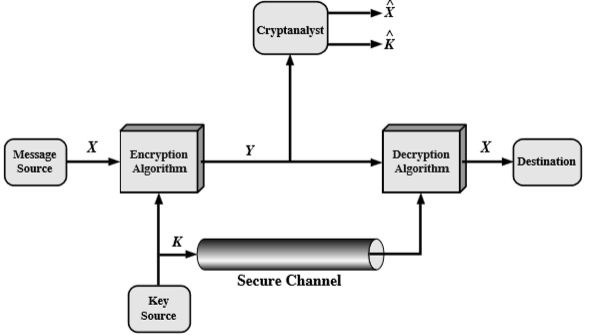
\includegraphics[width=0.45\textwidth]{Immagini/chiavesimmetrica.png}
    \end{center}
    Dove nel canale sicuro si invia la chiave e $\hat{X}$ è parte del messaggio decriptato e $\hat{K}$ è parte della chiave decriptata.
    \item Algoritmi Asimmetrici: le due chiavi sono diverse e non è possibile derivare una dall'altra e una chiave pubblica (\textbf{public key}) può essere distribuita senza compromettere le chiavi private (\textbf{private key})
    \item Quando si costruisce un sistema crittografico bisogna presumere che l'algoritmo sia conosciuto, quindi la sicurezza dipende dalla chiave
\end{itemize}
\section{Classificazione della sicurezza}
\begin{itemize}
    \item \textbf{Unconditional Security}: il sistema è sicuro anche se l'avversario ha potenza computazionale illimitata. La sicurezza è misurata in termini di teoria dell'informazione (information theory).
    \item \textbf{Conditional Security}: il sistema può essere violato se l'avversario ha abbastanza potenza computazionale. La sicurezza è misurata in termini di teoria della complessità (complexity theory).
\end{itemize}
\section{Criptoanalisi}
E' la scienza del recuperare il messaggio originale da quello criptato senza la chiave. L'obiettivo non è solo quello di recuperare il messaggio ma anche la chiave.
\subsection{Brute-force attack}
\begin{itemize}
    \item E' sempre possibile: basta provare tutte le chiavi, solitamente sono $2^{\#bit}$ chiavi possibili se sono caratteri invece è una permutazione di $n!$ chiavi possibili.
    \item Costa molto, dipende dalla dimensione della chiave
    \item Presume che il messaggio decifrato sia conociuto o riconoscibile
\end{itemize}
\subsection{Tipi di attacco}
\begin{itemize}
    \item \textbf{Ciphertext only}: l'aavversario conosce il testo cifrato e prova a dedurne la chiave
    \item \textbf{Known plaintext}: rispetto a ciphertext only, l'avversario conosce anche il testo decifrato
    \item \textbf{Chosen plaintext}: come sopra ma l'avversario può scegliere il testo cifrato
    \item \textbf{Adaptive chosen plaintext}: può, non solo scegliere il testo decifrato, ma può modificare il testo decifrato in base ai risultati della cifratura
    \item \textbf{Chosen ciphertext}: l'avversario può scegliere il testo cifrato e vedere il testo decifrato
\end{itemize}
\section{Matematicamente}
\begin{itemize}
    \item $\mathcal{A}$ è l'alfabeto, un insieme finito
    \item $\mathcal{M}\subseteq \mathcal{A}^{*}$ è lo spazio dei messaggi. $M\in \mathcal{M}$ è un messaggio in chiaro
    \item $\mathcal{C}$ è lo spazio dei testi cifrati, il cui alfabeto può essere diverso da quello di $\mathcal{M}$
    \item $\mathcal{K}$ denota l'insieme delle chiavi
    \item $e \in \mathcal{K}$ deterima una funzione biettiva $e: \mathcal{M} \rightarrow \mathcal{C}$, la funzione di cifratura è denotata da $E_{e}$
    \item $\forall d \in \mathcal{K}, D_{d}: \mathcal{C} \rightarrow \mathcal{M}$, la funzione di decifratura è denotata da $D_{d}$ ed è biettiva
    \item $D_{d}(E_{e}(M)) = E^{-1}_{e}(M) = M$
\end{itemize}
\section{Cifrari a blocchi, a flusso e a codici}
\begin{itemize}
    \item \textbf{Block cipher}: è uno schema di cifratura che divide il messaggio in blocchi di lunghezza fissa $t$ e cifra ogni blocco separatamente.
    \item \textbf{Stream cipher}: è uno schema di cifratura dove il blocco è di lunghezza 1 (un bit alla volta)
    \item \textbf{Code}: è uno schema di cifratura dove il messaggio è cifrato in blocchi di lunghezza variabile
\end{itemize}
\section{Cifrari a sostituzione}
\begin{itemize}
    \item \textbf{Cifrario di Cesare}: ogni carattere del messaggio in chiaro viene sostituito dal carattere $n$ a destra modulo 26 (26! possibili chiavi, molto poco sicuro)
    \item \textbf{ROT13}: è un cifrario di Cesare con $n=13$
    \item \textbf{Alfanumerico}: si sostituisce ogni carattere con un numero
\end{itemize}
\subsection{Esempio: Cifrario affine}
\begin{itemize}
    \item E' una sostituzione monoalfabetica tale che $E(m)=(a\cdot m+b) \mod |\mathcal{A}|$ dove a,b sono interi positivi e sono chiave del cifrario
    \item Per essere invertibile $a$ deve essere coprimo con $|\mathcal{A}|$
    \item La decifratura è $D(c) = a^{-1}(c-b) \mod |\mathcal{A}|$ dove $1 = a\cdot a^{-1}\mod |\mathcal{A}|$
\end{itemize}
\subsection{Cifrario a sostituzione omofono}
Sostituisce ogni lettera $a$ con una stringa scelta a caso da $H(a)$. Per decifrare una stringa $c$ di $t$ simboli, bisogna determinare $a$ tale che $H(a)=c$. La chiave del cifrario è la funzione $H$.
\subsubsection{Esempio}
\begin{itemize}
    \item $H(A)=\{1,2\}$
    \item $H(B)=\{3,4\}$
    \item $H(C)=\{5,6\}$
\end{itemize}
ABC $\rightarrow$ 135 oppure 246 oppure 145 ecc.
\subsection{Cifrario a sostituzione polialfabetica}
E' un cifrario a blocchi con lunghezza t sull'alfabeto A
\subsection{One-time pads (cifrario di Vernam)}
E' un cifrario a flusso definito sull'alfabeto $\mathcal{A}=\{0,1\}$  il messaggio è cifrato scegliendo casualmente una chiave $k$ binaria di lunghezza uguale al messaggio $m$ e facendo $c=m\oplus k$ dove $\oplus$ è l'operazione di XOR, $d=c\oplus k$ è la decifratura.\\
\underline{Le chiavi non vanno mai riutilizzate}.\\
La funzione di cifratura $E(K,M)$ è \textbf{malleabile} se e solo se
\begin{equation*}
    F(E(K,M)) = E(K,G(M)) \quad\forall K,M
\end{equation*}
\subsubsection{Esempio}
La funzione $E(K,M)=K\oplus M$ è chiaramente malleabile. Se $F(X)=G(X)=N\oplus X$
\begin{equation*}
    F(E(K,M)) = N\oplus (K\oplus M) = K \oplus (N\oplus M) = E(K,N\oplus M) = E(K,G(M))
\end{equation*}
\subsection{Cifrario a trasposizione}
E' un cifrario che "mischia" (permutazione) le lettere del messaggio senza cambiarne il significato (delle lettere) (es. CIAO $\rightarrow$ OICA) per decifrare bisogna eseguire l'operazione inversa della permutazione.
\subsection{Cifrario composito}
I cifrari basati su sostituzione e trasposizione non sono sicuri però possono essere combinati, è difficile farlo "a mano" infatti sono state inventate le macchine cifranti.
\chapter{Crittografia simmetrica}
\section{Cifrario Feistel}
\begin{center}
    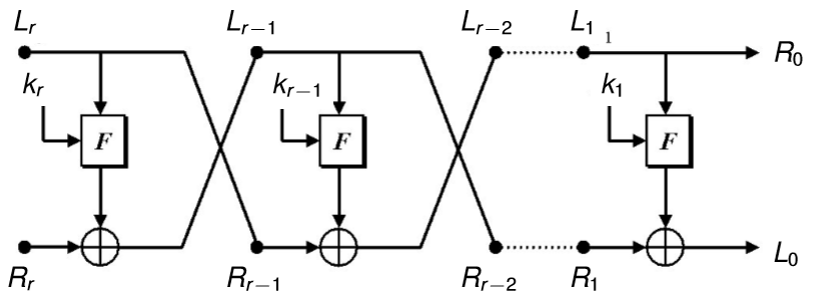
\includegraphics[width=\textwidth]{Immagini/feistelc.png}
\end{center}
$F$ è la funzione di cifratura, lavora sempre con il blocco sinistro del messaggio ed esegue lo \texttt{XOR}.\\
La struttura della cifratura e deicfratura è la stessa, la differenze è che le sotto-chiavi usate durante la cifratura a ogni round sono usate in ordine inverso durante la decifratura.
\begin{center}
    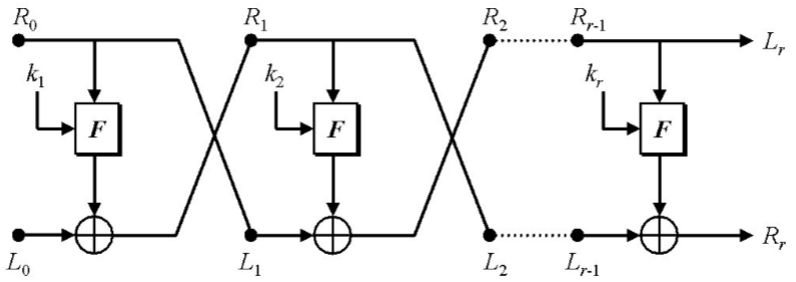
\includegraphics[width=\textwidth]{Immagini/feisteld.png}
\end{center}
\begin{equation*}
    R_{r}\oplus L_{r-1} = F(k_{r},R_{r-1})
\end{equation*}
\chapter{Crittografia simmetrica}
\chapter{Message auth \& Digital signature}
\chapter{Public key cryptography}
\chapter{Security protocols}
\chapter{Web security}
\end{document}